\documentclass[10pt]{article}
\usepackage[T1]{fontenc}
\usepackage{amsmath, amsfonts, amssymb}
\usepackage{geometry}
\geometry{a4paper, margin=1in} % Fixes the overfull \hbox and \vbox warnings
\usepackage[version=4]{mhchem}
\usepackage{graphicx}
\usepackage[export]{adjustbox}
\usepackage{caption}
\usepackage{bbold}
\usepackage{booktabs}

% --- TikZ Setup for Advanced Diagrams ---
\usepackage{tikz}
\usetikzlibrary{patterns, arrows.meta, positioning, calc}

\allowdisplaybreaks % Allows equations to break across pages cleanly

\begin{document}
\captionsetup{singlelinecheck=false}

$u=a_{1} x+a_{2} x^{2}$. After substituting into Eq. 3.5-3 and writing $\frac{\partial \Pi_{p}}{\partial a_{1}}=0$ and $\frac{\partial \Pi_{p}}{\partial a_{2}}=0$, we obtain

\begin{align*}
A E L_{T}\begin{bmatrix}
1 & L_{T} \\
L_{T} & 4 L_{T}^{2} / 3
\end{bmatrix}\begin{Bmatrix}
a_{1} \\
a_{2}
\end{Bmatrix} &= \frac{c L_{T}^{3}}{12}\begin{Bmatrix}
4 \\
3 L_{T}
\end{Bmatrix} \quad \text{or} \quad \begin{Bmatrix}
a_{1} \\
a_{2}
\end{Bmatrix} = \frac{c L_{T}}{12 A E}\begin{Bmatrix}
7 L_{T} \\
-3
\end{Bmatrix} \\
\text{hence} \quad u &= \frac{c L_{T}}{12 A E}\left(7 L_{T} x-3 x^{2}\right) \quad \text{and} \quad \sigma_{x}=E u_{,x}=\frac{c L_{T}}{12 A}\left(7 L_{T}-6 x\right) \tag{3.5-6b}
\end{align*}

Figures 3.5-1 $b$ and 3.5-1 c show the comparison between exact and approximate results. As might be expected, the two-term results (Eqs. 3.5-6) are better than the one-term results (Eqs. 3.5-5). With the body force term $F_{x}=c x / A$, the differential equation of equilibrium (Eq. 1.6-2a) becomes

\begin{equation*}
\sigma_{x, x}+\frac{c x}{A}=0 \quad \text { or } \quad A E u_{, x x}+c x=0 \tag{3.5-7}
\end{equation*}

The latter equation results from the substitution $\sigma_{x}=E u,_{x}$. Neither Eq. 3.5-7, nor the natural boundary condition $\sigma_{x}=0 \text{ at } x=L_{T}$, is satisfied by the foregoing two approximate solutions.

Notice that approximate displacements are more accurate than approximate stresses. This is to be expected, because stresses are calculated from derivatives of the approximating field. (To see that differentiation emphasizes discrepancies, consider the functions $f_{1}=4 x(1-x)$ and $f_{2}=\sin \pi x$. In the range $0<x<1$, functions $f_{1}$ and $f_{2}$ look much alike, but successive derivatives of $f_{1}$ and $f_{2}$ have less and less resemblance.)

The exact solution of the problem of Fig. 3.5-1a is

\begin{equation*}
u=\frac{c}{6 A E}\left(3 L_{T}^{2} x-x^{3}\right) \tag{3.5-8}
\end{equation*}

Use of the series $u=a_{1} x+a_{2} x^{2}+a_{3} x^{3}$ in the Rayleigh-Ritz method produces

\begin{equation*}
a_{1}=\frac{c L_{T}^{2}}{2 A E} \quad a_{2}=0 \quad a_{3}=-\frac{c}{6 A E} \tag{3.5-9}
\end{equation*}

which is the exact solution. Use of still more terms leads again to the exact solution: one finds $a_{1}, a_{2}$, and $a_{3}$ to be the values given in Eq. 3.5-9 and $a_{4}=a_{5}=a_{6}=\cdots= a_{n}=0$. In general, the Rayleigh-Ritz method yields the exact solution if the approximating field is capable of representing the exact field by appropriate choice of d.o.f. $a_{j}$. In practice this circumstance is rare.

\subsection*{3.6 COMMENTS ON THE \\
 RAYLEIGH-RITZ METHOD BASED ON ASSUMED DISPLACEMENT FIELDS}

Approximating fields must be admissible and should be easy to use. Only polynomials, and occasionally sine and cosine functions, are simple enough to be practicable. Beyond this there are no easy answers to important questions: What sort of assumption for the field is best? What particular terms and how many of them? How good are the computed results? These difficulties and uncertainties are increased for multidimensional problems.

Let a problem be solved repeatedly, each time with another term added to the assumed field (as in Eqs. 3.5-5 and 3.5-6, for example). Thus we generate a sequence of trial solutions. We expect the sequence to converge: to the exact $\Pi_{p}$, to the exact displacements, and to the exact stresses. A necessary condition for convergence is that trial field be complete.

Completeness is achieved if the exact displacements, and their derivatives that appear in $\Pi_{p}$, can be matched arbitrarily closely if enough terms appear in the trial field. A polynomial series is complete if it is of high enough degree and if no terms are omitted. Fourier series are also complete.

Completeness demands that the lowest-order admissible terms be included. For example, consider the end-loaded bar of Fig. 3.4-2. If we omit the term $a_{1} x$ from Eq. $3.5-4$, we omit the very term that contains the exact answer-namely, $u=$ (P/AE)x. Thus completeness is destroyed, and the sequence of approximate solution does not produce the exact answer even if the number of terms approaches infinity. This is easy to see: if Eq. 3.5-4 begins with $a_{2} x^{2}$, then $\sigma_{x}=E u_{,x}=0$ at $x=0$, which is incorrect. The term $a_{1} x$ represents the essential constant-strain capability. (In a finite element context, this requirement means that each element must be capable of representing a state of constant strain.)

Completeness also requires that no series terms be omitted. Referring again to Eq. 3.5-4, a two-term approximation should be $a_{1} x+a_{2} x^{2}$ but not $a_{1} x+a_{3} x^{3}$, and not $a_{1} x+a_{4} x^{4}$, and so on.

In two dimensions, a polynomial is of degree $n$ if it contains a term of the form $x^{\ell} y^{m}$, where $\ell$ and $m$ are nonnegative integers and $\ell+m=n$. The polynomial is complete if it contains all combinations of $\ell$ and $m$ for which $\ell+m=n$ and if no lower-order terms are omitted. For example, a complete quadratic, $n=2$, has the form $u=a_{1}+a_{2} x+a_{3} y+a_{4} x^{2}+a_{5} x y+a_{6} y^{2}$. A complete polynomial of degree $n$ in two dimensions contains $(n+1)(n+2) / 2$ terms (see Fig. 3.6-1).

In three dimensions, similar remarks apply, so that a complete quadratic contains 10 terms, which include a constant term, the linear terms $x, y$, and $z$, and the quadratic terms $x^{2}, x y, y^{2}, y z, z^{2}$, and $z x$.

A Rayleigh-Ritz solution is either exact or it is too stiff. This happens because the mathematical structure is permitted to displace only into shapes that can be described by superposing the finite number of functions $f_{i}$ present in the assumed displacement field that the analyst selects. Therefore, the correct shape is excluded, unless the assumed field happens to contain it. Effectively, the assumed field imposes constraints that prevent the structure from deforming the way it wants to. Constraints stiffen a structure. In effect, the solution method creates a substitute structure that is stiffer than the real one.

The work $W$ done by loads that gradually increase from zero to $\{\mathbf{R}\}$ is $W= \{\mathbf{D}\}^{T}\{\mathbf{R}\} / 2$ if the structure is linearly elastic. An approximate solution yields d.o.f.

\begin{figure}[htbp]
\begin{center}
    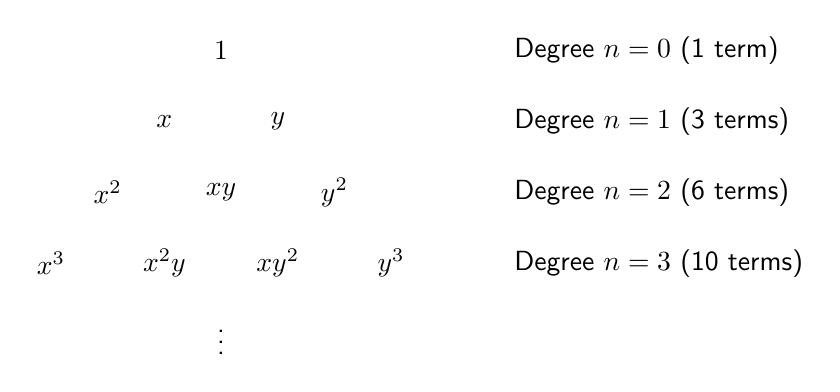
\begin{tikzpicture}[font=\sffamily, scale=0.9]
        % Node alignments for Pascal's triangle
        \node at (0, 0) {$1$};
        \node[right] at (4, 0) {Degree $n=0$ (1 term)};

        \node at (-0.8, -1) {$x$}; 
        \node at (0.8, -1) {$y$};
        \node[right] at (4, -1) {Degree $n=1$ (3 terms)};

        \node at (-1.6, -2) {$x^2$}; 
        \node at (0, -2) {$xy$}; 
        \node at (1.6, -2) {$y^2$};
        \node[right] at (4, -2) {Degree $n=2$ (6 terms)};

        \node at (-2.4, -3) {$x^3$}; 
        \node at (-0.8, -3) {$x^2y$}; 
        \node at (0.8, -3) {$xy^2$}; 
        \node at (2.4, -3) {$y^3$};
        \node[right] at (4, -3) {Degree $n=3$ (10 terms)};
        
        \node at (0, -4) {$\vdots$};
    \end{tikzpicture}
\captionsetup{labelformat=empty}
\caption{Figure 3.6-1. Pascal triangle, showing the number of terms in complete polynomials in two independent variables $x$ and $y$.}
\end{center}
\end{figure}

\{\textbf{D}\} such that work $W$ is less than the exact value. This does not necessarily mean that every d.o.f. in $\{\mathbf{D}\}$ is underestimated. But if the structure carries a single load $P$, we can say that its computed displacement $D$ is a lower bound to the correct magnitude.

Strain energy $U$ is numerically equal to $W$, so the approximate solution underestimates $U$ when loads are prescribed. If displacements are prescribed instead, $U$ is overestimated because extra force is needed to deform an overly stiff structure. When loads and displacements are prescribed, $U$ may be high or low.

Stresses are calculated from displacements, so we expect that a too-stiff structure will underestimate stress magnitudes. However, as seen in Fig. 3.5-1c, approximate stresses may be too low in one place but too high in another, even when the stress is derived from an approximate displacement field that is everywhere too low. Accordingly, a rule about stress magnitudes would be either so crude or so equivocal as to be of little value.

\subsection*{3.7 STATIONARY PRINCIPLES AND GOVERNING EQUATIONS}

The principle of stationary potential energy is but one of many stationary principles of mathematical physics. Central to each is a functional, of which $\Pi_{p}$ is but one. Rayleigh-Ritz approximations and finite element formulations can be derived from functionals. For this reason the following brief remarks are offered.

Consider the functional for $\Pi_{p}$, Eq. 3.4-1. It depends on displacements $\{\mathbf{u}\}$ and on strains $\{\boldsymbol{\epsilon}\}$, which are derivates of $\{\mathbf{u}\}$. The term "functional" indicates that $\Pi_{p}$ depends not on $\{\mathbf{u}\}$ and its derivatives at a point but upon their integrated effect over a region of interest. The stationary condition $d \Pi_{p}=0$ may be applied directly to Eq. 3.4-1, without first expressing $\Pi_{p}$ in terms of a finite number of d.o.f. This is accomplished by using the calculus of variations, the procedures of which are beyond the scope of this book [3.1]. However, the end results of setting $d \Pi_{p}$ to zero are found to be the differential equations of equilibrium (Eqs. 1.6-2) and the nonessential boundary conditions (the stress boundary conditions, Eqs. 1.6-4). Thus, if the field $\{\mathbf{u}\}$ is admissible, the statement $d \Pi_{p}=0$ implies all components of a valid solution: satisfaction of equilibrium, compatibility, and boundary conditions. In an approximate solution, equilibrium conditions and stress boundary conditions are satisfied only in an average or integral sense, not at every point.

In other physical problems there exist other functionals $\Pi$. Instead of displacements $\{\mathbf{u}\}$, the primary field may be temperature, or pressure, or voltage, and so on. In each case the functional $\Pi$ can be tested for correctness by applying the calculus of variations to see if the condition $d \Pi=0$ yields the appropriate governing differential equation and nonessential boundary conditions.

Boundary Conditions. In order to use variational methods, one must be able to distinguish between essential and nonessential boundary conditions. For a problem having one dependent field variable, the rule is as follows. Let $2 m$ be the highest-order derivative of the dependent field variable in the governing differential equation. (Derivatives of order $m$ then appear in the functional.) Essential boundary conditions involve derivatives of order zero through $m-1$, the zeroth derivative being the dependent variable itself. Nonessential boundary conditions involve derivatives of order $m$ and higher, up to and including $2 m-1$. The following are examples.

\begin{center}
\noindent\adjustbox{max width=\textwidth}{
\begin{tabular}{lllr}
\toprule
\multicolumn{1}{c}{Problem} & \multicolumn{1}{c}{Bar (Fig. 3.5-1a)} & \multicolumn{1}{c}{Beam bending} & \multicolumn{1}{c}{\begin{tabular}[c]{@{}c@{}}Two-dimensional \\ heat conduction\end{tabular}} \\
\midrule
Differential equation & $A E u_{, x x}+q=0$ & $E I w_{, x x x x}-q=0$ & $k \nabla^{2} T+Q=\rho c \dot{T}$ \\
$2 m, m-1,2 m-1$ & $2,0,1$ & $4,1,3$ & $2,0,1$ \\
Essential B.C. & On $u$ only & On $w$ and $w_{, x}$ & On $T$ only \\
Nonessential B.C. & On $\sigma_{x}=E u_{, x}$ & On $M=E I w_{, x x}$ & On $q=-k(T_{, x} \ell_{B}$ \\
 & & and $V=E I w_{, x x x}$ & $\left.+T_{,y} m_{B}\right)$ \\
\bottomrule
\end{tabular}
}
\end{center}

In these examples the dependent field variables are axial displacement $u$, lateral displacement $w$, and temperature $T$. Nonessential boundary conditions concern axial stress $\sigma_{x}$, bending moment $M$, transverse shear force $V$, and heat flow $q$. In the heat conduction example, $k$ is thermal conductivity, $\dot{T}$ means the time derivative of $T$, and $\ell_{B}$ and $m_{B}$ are direction cosines of a normal to the boundary (see Chapter 16).

The foregoing remarks are little changed if there is more than one field. Imagine, for example, that there are dependent field variables $u$ and $v$, with second derivatives $u_{,x x}, u_{,xy}, u_{,yy}, v_{,xx}, v_{,xy}$, and $v_{,yy}$ in the governing differential equations and first derivatives $u_{,x}, u_{,y}, v_{,x}$ and $v_{,y}$ in the functional. Then $2m=2$ and $m=1$ for both $u$ and $v$. Essential boundary conditions are prescriptions of $u$ and $v$ at particular locations. Nonessential boundary conditions involve first derivatives of $u$ and $v$, either singly or in combination.

Functionals and Governing Differential Equations. Imagine that a functional $\Pi$ depends on two dependent field variables, $u=u(x, y)$ and $v=v(x, y)$, in which independent variables $x$ and $y$ are Cartesian coordinates:

\begin{equation*}
\Pi=\iint F\left(x, y, u, v, u_{,x}, u_{,y}, v_{,x}, v_{,y}, \ldots, v_{,yy}\right) d x d y \tag{3.7-1}
\end{equation*}

Here we will assume that $F$ contains no derivatives of order higher than second. There are as many "Euler equations" as there are dependent field variables. An Euler equation is a governing differential equation of the physical problem. Methods of calculus of variations extract from Eq. 3.7-1 the Euler equations

\begin{align*}
& \frac{\partial F}{\partial u}-\frac{\partial}{\partial x} \frac{\partial F}{\partial u_{,x}}-\frac{\partial}{\partial y} \frac{\partial F}{\partial u_{,y}}+\frac{\partial^{2}}{\partial x^{2}} \frac{\partial F}{\partial u_{,x x}}+\frac{\partial^{2}}{\partial x \partial y} \frac{\partial F}{\partial u_{,x y}}+\frac{\partial^{2}}{\partial y^{2}} \frac{\partial F}{\partial u_{,y y}}=0  \tag{3.7-2a}\\
& \frac{\partial F}{\partial v}-\frac{\partial}{\partial x} \frac{\partial F}{\partial v_{,x}}-\frac{\partial}{\partial y} \frac{\partial F}{\partial v_{,y}}+\frac{\partial^{2}}{\partial x^{2}} \frac{\partial F}{\partial v_{,x x}}+\frac{\partial^{2}}{\partial x \partial y} \frac{\partial F}{\partial v_{,xy}}+\frac{\partial^{2}}{\partial y^{2}} \frac{\partial F}{\partial v_{,yy}}=0 \tag{3.7-2b}
\end{align*}

Equations 3.7-1 and 3.7-2 both describe the same problem, Eq. 3.7-1 being called the "weak form" and Eqs. 3.7-2 the "strong form."

As a specific example of Eq. 3.7-2, consider the axially loaded uniform bar described by Fig. 3.5-1a. Here there is one independent variable, one dependent variable, and no second derivative. Equation 3.7-1 reduces to Eq. 3.5-3. There is but one Euler equation, Eq. 3.7-2a, which reduces to

\begin{equation*}
\frac{\partial F}{\partial u}-\frac{d}{d x} \frac{\partial F}{\partial u_{, x}}=0 \quad \text { in which } \quad F=\frac{1}{2} A E u_{, x}^{2}-u(c x) \tag{3.7-3}
\end{equation*}

Derivatives in the Euler equation are

\begin{equation*}
\frac{\partial F}{\partial u}=-c x \quad \text { and } \quad \frac{d}{d x} \frac{\partial F}{\partial u_{, x}}=\frac{d}{d x}\left(A E u_{, x}\right)=A E u_{, x x} \tag{3.7-4}
\end{equation*}

from which Eq. 3.5-7 is obtained, as expected.

As another example, consider plane heat conduction in an isotropic material. A suitable functional is

\begin{equation*}
\Pi=\iint\left(\frac{1}{2} k T^{2}_{,x}+\frac{1}{2} k T^{2}_{,y}-Q T+\rho c T \dot{T}\right) d x d y \quad \text { or } \quad \Pi=\iint F d x d y \tag{3.7-5}
\end{equation*}

in which $T=$ temperature, $k=$ thermal conductivity, $Q=$ internally generated heat flow, $\rho=$ mass density, $c=$ specific heat, and $\dot{T}$ is the time derivative $\partial T / \partial t$. Unit thickness is assumed. (Equation 3.7-5 omits certain boundary terms of practical interest. See Section 16.3 for a more detailed treatment.) Again there is one dependent field variable, $T$, and one Euler equation-namely,

\begin{equation*}
\frac{\partial F}{\partial T}-\frac{\partial}{\partial x} \frac{\partial F}{\partial T_{, x}}-\frac{\partial}{\partial y} \frac{\partial F}{\partial T_{, y}}=0 \tag{3.7-6}
\end{equation*}

where $F$ is the integrand of Eq. 3.7-5. Equations 3.7-5 and 3.7-6 yield

\begin{equation*}
k\left(T_{, x x}+T_{, y y}\right)+Q-\rho c \dot{T}=0 \tag{3.7-7}
\end{equation*}

as the differential equation that describes the temperature distribution in the region of interest.

Potential energy functionals $\Pi_{p}$ for problems of beam bending and plate bending contain second derivatives of lateral displacement $w$. These and other examples are left as exercises.

The calculus of variations also produces natural boundary conditions. An explanation of their derivation and interpretation takes more space than we can allot to it. The reader is referred to other texts [3.1,3.2].

Finally, we remark that although there is always a differential equation associated with a functional, the reverse is not necessarily true. For example, a differential equation that contains an odd-numbered derivative does not have an associated functional of the form of Eq. 3.7-1.

Variational Methods: A Brief Example. Figure 3.7-1 shows a uniform bar loaded by distributed axial load $q=q(x)$ and prescribed stress $\sigma_{L}$ at $x=L$. We will use this problem to illustrate that the calculus of variations produces the governing differential equation and the nonessential boundary condition. In this way we will discover the origin of terms seen in Eqs. 3.7-3 and 3.7-4. The development will

\begin{figure}[htbp]
\begin{center}
    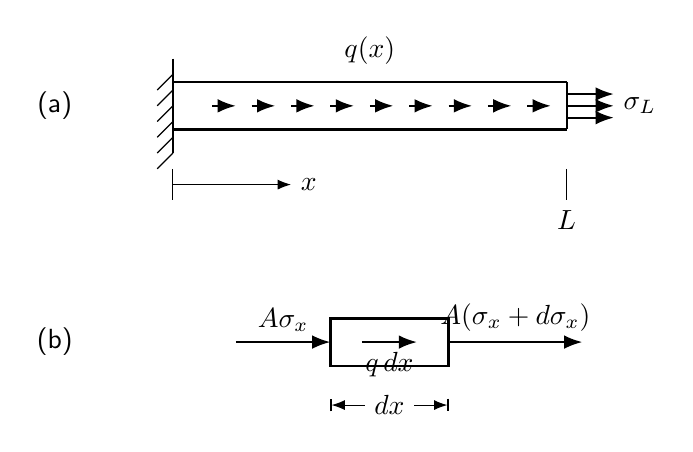
\begin{tikzpicture}[>=Latex, font=\sffamily]
        % Part (a)
        \node at (-1.5, 0) {(a)};
        % Wall
        \draw[thick] (0, 0.6) -- (0, -0.6);
        \foreach \y in {-0.6, -0.4, ..., 0.6} { \draw (0,\y) -- (-0.2,\y-0.2); }
        % Bar
        \draw[thick] (0, 0.3) -- (5, 0.3);
        \draw[thick] (0, -0.3) -- (5, -0.3);
        \draw[thick] (5, 0.3) -- (5, -0.3);
        % Distributed Load
        \foreach \x in {0.5, 1.0, ..., 4.5} { \draw[->, thick] (\x, 0) -- (\x+0.3, 0); }
        \node[above] at (2.5, 0.4) {$q(x)$};
        % End Stress
        \foreach \y in {0.15, 0, -0.15} { \draw[->, thick] (5, \y) -- (5.6, \y); }
        \node[right] at (5.6, 0) {$\sigma_L$};
        % Coordinate Axis
        \draw[->] (0, -1) -- (1.5, -1) node[right] {$x$};
        \draw (0, -0.8) -- (0, -1.2);
        \draw (5, -0.8) -- (5, -1.2) node[below] {$L$};

        % Part (b)
        \begin{scope}[shift={(0, -3)}]
            \node at (-1.5, 0) {(b)};
            % Element
            \draw[thick] (2, 0.3) rectangle (3.5, -0.3);
            % Left Stress
            \draw[->, thick] (0.8, 0) -- (2, 0) node[midway, above] {$A\sigma_x$};
            % Right Stress
            \draw[->, thick] (3.5, 0) -- (5.2, 0) node[midway, above] {$A(\sigma_x + d\sigma_x)$};
            % Distributed Load inside
            \draw[->, thick] (2.4, 0) -- (3.1, 0) node[midway, below] {$q \, dx$};
            % Dimension dx
            \draw[|<->|] (2, -0.8) -- (3.5, -0.8) node[midway, fill=white] {$dx$};
        \end{scope}
    \end{tikzpicture}
\captionsetup{labelformat=empty}
\caption{Figure 3.7-1. (a) Uniform elastic bar loaded by distributed axial load $q$ and end stress $\sigma_{L}$. (b) Forces that act on a differential element of the bar.}
\end{center}
\end{figure}

also be seen to produce the virtual work equation and to suggest an alternative formulation method (the method of weighted residuals).

In Eq. 3.4-6, let $\epsilon_{x}=u,_{x}, F_{x}=q / A, D=u_{L}$, and $P=A \sigma_{L}$. Thus the potential energy functional for the bar in Fig. 3.7-1a is

\begin{equation*}
\Pi_{p}=\frac{A E}{2} \int_{0}^{L} u_{, x}^{2} d x-\int_{0}^{L} q u d x-\left(A \sigma_{L}\right) u_{L} \tag{3.7-8}
\end{equation*}

We presume that $u=u(x)$ is an admissible displacement field for this problemthat is, a field that is continuous and satisfies the essential boundary condition $u=0$ at $x=0$. Let $u$ be perturbed by an amount $\delta u$, which we elect to write as $\delta u=e \eta$, where $e$ is a small number and $\eta=\eta(x)$ is an admissible field. Thus the perturbed field $u+e \eta$ is also admissible and satisfies the same essential boundary condition as $u$. Hence, $u_{, x}$ becomes $u_{, x}+e \eta_{, x}, u_{L}$ becomes $u_{L}+e \eta_{L}$, and $\Pi_{p}$ becomes $\Pi_{p}+\delta \Pi_{p}$. The change in energy $\left(\Pi_{p}+\delta \Pi_{p}\right)-\Pi_{p}$ is

\begin{equation*}
\delta \Pi_{p}=e\left[A E \int_{0}^{L} u_{,x} \eta_{, x} d x-\int_{0}^{L} q \eta d x-\left(A \sigma_{L}\right) \eta_{L}\right]+e^{2} \frac{A E}{2} \int_{0}^{L} \eta_{, x}^{2} d x \tag{3.7-9}
\end{equation*}

According to the potential energy principle, stable equilibrium occurs when $\Pi_{p}$ is a relative minimum. This implies that $\delta \Pi_{p}>0$ for any admissible $\eta$. Now $e^{2} \eta_{, x}^{2}$ is never negative, and the remaining term $e[\cdots]$ changes sign when $e$ changes sign. We conclude that if $\delta \Pi_{p}$ is to be positive for all small values of $e$, the bracketed expression in Eq. 3.7-9 must vanish. Setting this expression to zero, and integrating its first term by parts according to the standard formula $\int u d v=-\int v d u+ \omega v$, we obtain

\begin{equation*}
0=-A E \int_{0}^{L} u_{, x x} \eta d x+\left[A E u_{, x} \eta\right]_{0}^{L}-\int_{0}^{L} q \eta d x-\left(A \sigma_{L}\right) \eta_{L} \tag{3.7-10}
\end{equation*}

But $\eta=0$ at $x=0$, so Eq. 3.7-10 becomes

\begin{equation*}
0=-\int_{0}^{L}\left(A E u_{, x x}+q\right) \eta d x+A\left(E u_{, x}-\sigma_{L}\right) \eta_{L} \tag{3.7-11}
\end{equation*}

Since $\eta=\eta(x)$ is admissible but otherwise arbitrary, an arbitrary value of $\eta_{L}$ can be assigned while infinitely many functions $\eta$ are yet possible in the range $0 < x < L$. Accordingly, Eq. 3.7-11 can be satisfied only if the coefficients of $\eta$ and $\eta_{L}$ vanish separately. Thus we obtain

\begin{align*}
A E u_{, x x}+q=0 & \text { for } 0<x<L  \tag{3.7-12a}\\
E u_{, x}-\sigma_{L}=0 & \text { at } x=L \tag{3.7-12b}
\end{align*}

Equation 3.7-12a is the governing differential equation. It can be written in the alternative form $A \sigma_{x, x}+q=0$, and can also be derived by considering the equilibrium of axial forces in Fig. 3.7-1b. Equation 3.7-12b is a nonessential (or natural) boundary condition, which says that $\epsilon_{x}=\sigma_{L} / E$ at $x=L$.

The vanishing of the bracketed expression in Eq. 3.7-9 can be regarded as an expression of the virtual work principle, which states that the total work of internal and external forces must vanish for any admissible infinitesimal displacement from an equilibrium configuration. In Eq. 3.7-9 internal forces $A E u_{, x} d x=A \sigma_{x} d x$ do work (and store strain energy) when strains $\eta_{, x}$ occur, and external forces $q d x$ and $A \sigma_{L}$ do negative work (and lose potential energy) when positive displacements $\eta$ and $\eta_{L}$ occur.

Matrices used in finite element analysis can be generated from either Eq. 3.7-8 or the bracketed expression in Eq. 3.7-9. (In Eq. 3.7-9, if we identify $u_{, x}$ as $\epsilon_{x}$ and $e \eta_{,x}$ as $\delta \epsilon_{x}$, the first integrand becomes $\delta \epsilon_{x} A E \epsilon_{x}$, which will subsequently be recognized as a familiar form.)

The vanishing of the bracketed expression in Eq. 3.7-9 can also be obtained by "working backward," as follows. Imagine that we seek an approximate solution $\bar{u}=\bar{u}(x)$-for example, the admissible polynomial $\bar{u}=a_{1} x+a_{2} x^{2}+a_{3} x^{3} + \cdots$, where the $a_{i}$ are constants that must be determined. Now $\bar{u}$ does not satisfy Eq. 3.7-12a for all $x$ : a "residual," $R=R(x)=A E \bar{u}_{, x x}+q \neq 0$, is left over. Nevertheless, we can select the $a_{i}$ so as to satisfy Eq. 3.7-12a in an average or integral sense by writing

\begin{equation*}
\int_{0}^{L}\left(A E \bar{u}_{, x x}+q\right) \eta d x=0 \tag{3.7-13}
\end{equation*}

where $\eta=\eta(x)$ may now be called a "weight function." Applying integration by parts to Eq. 3.7-13, we obtain

\begin{equation*}
-A E \int_{0}^{L} \bar{u}_{, x} \eta_{, x} d x+[A E \bar{u}_{, x} \eta]_{0}^{L}+\int_{0}^{L} q \eta d x=0 \tag{3.7-14}
\end{equation*}

But $\eta=0$ at $x=0$. In addition, at $x=L$, we may replace $E u_{, x}$ by $\sigma_{L}$, thus introducing the nonessential boundary condition. Equation 3.7-14 becomes

\begin{equation*}
-A E \int_{0}^{L} \bar{u}_{, x} \eta_{, x} d x+\int_{0}^{L} q \eta d x+\left(A \sigma_{L}\right) \eta_{L}=0 \tag{3.7-15}
\end{equation*}

which agrees with the vanishing of the bracketed expression in Eq. 3.7-9. This method of formulating a problem for approximate solution is called a weighted residual method. It can be applied to problems for which one knows the differential equation but not the functional or the variational principle. If $\eta_{i}=\partial \bar{u} / \partial a_{i}$ the method is known as the Galerkin method (for which Eq. 3.7-15 yields as many
equations as there are $a_{i}$ to be determined). A more detailed discussion appears in Chapter 15.

\subsection*{3.8 A PIECEWISE POLYNOMIAL FIELD}
In this section we use a one-dimensional example to illustrate how a displacement field can be written in terms of physical displacements $\{\mathbf{d}\}$ rather than parameters $a_{i}$ (as in Eq. 3.5-4). The use of $\{\mathbf{d}\}$, in combination with a piecewise polynomial field, leads to the finite element method in a form that is easy to program for computer solution. We begin by using the $a_{i}$, then show how to replace them by functions of nodal d.o.f. $d_{i}$.

Consider the bar of Fig. 3.8-1a. It is to be loaded axially. Axial displacement $u$ over the length from $x=0$ to $x=L_{T}$ is to be approximated as three separate linear fields,

\begin{align*}
u&=a_{1}+a_{2} x \quad \text{for } 0 \leqslant x \leqslant x_{2} \\
u&=a_{3}+a_{4} x \quad \text{for } x_{2} \leqslant x \leqslant x_{3} \\
u&=a_{5}+a_{6} x \quad \text{for } x_{3} \leqslant x \leqslant x_{4} \tag{3.8-1c}
\end{align*}

where the $a_{i}$ are d.o.f. to be determined in a subsequent Rayleigh-Ritz solution. For the field of Eqs. 3.8-1 to be admissible we must have $u=0$ at $x=0$. In addition, the first and second expressions must yield the same $u$ at $x=x_{2}$, and the second and third expressions must yield the same $u$ at $x=x_{3}$. These three conditions yield $a_{1}=0, a_{3}=\left(a_{2}-a_{4}\right) x_{2}$, and $a_{5}=\left(a_{2}-a_{4}\right) x_{2}+\left(a_{4}-a_{6}\right) x_{3}$. Thus Eqs. 3.8-1 assume the form

\begin{align*}
u &= a_{2} x \quad \text{for } 0 \leqslant x \leqslant x_{2} \\
u &= a_{2} x_{2}+a_{4}\left(x-x_{2}\right) \quad \text{for } x_{2} \leqslant x \leqslant x_{3} \\
u &= a_{2} x_{2}+a_{4}\left(x_{3}-x_{2}\right)+a_{6}\left(x-x_{3}\right) \quad \text{for } x_{3} \leqslant x \leqslant x_{4} \tag{3.8-2}
\end{align*}

\begin{figure}[htbp]
\begin{center}
    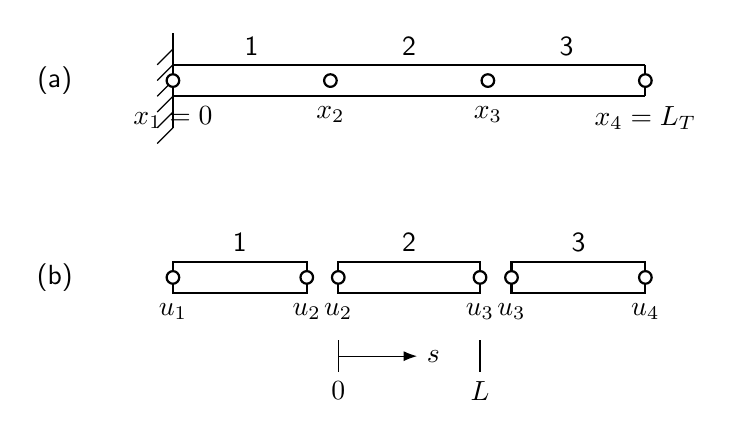
\begin{tikzpicture}[>=Latex, font=\sffamily]
        % Part (a)
        \node at (-1.5, 0) {(a)};
        % Wall
        \draw[thick] (0, 0.6) -- (0, -0.6);
        \foreach \y in {-0.6, -0.4, ..., 0.6} { \draw (0,\y) -- (-0.2,\y-0.2); }
        % Bar
        \draw[thick] (0, 0.2) -- (6, 0.2);
        \draw[thick] (0, -0.2) -- (6, -0.2);
        \draw[thick] (6, 0.2) -- (6, -0.2);
        
        % Nodes
        \filldraw[fill=white, draw=black, thick] (0,0) circle (0.08) node[below=0.2cm] {$x_1=0$};
        \filldraw[fill=white, draw=black, thick] (2,0) circle (0.08) node[below=0.2cm] {$x_2$};
        \filldraw[fill=white, draw=black, thick] (4,0) circle (0.08) node[below=0.2cm] {$x_3$};
        \filldraw[fill=white, draw=black, thick] (6,0) circle (0.08) node[below=0.2cm] {$x_4=L_T$};
        
        % Elements
        \node[above] at (1, 0.2) {1};
        \node[above] at (3, 0.2) {2};
        \node[above] at (5, 0.2) {3};

        % Part (b)
        \begin{scope}[shift={(0, -2.5)}]
            \node at (-1.5, 0) {(b)};
            % Element 1
            \draw[thick] (0, 0.2) rectangle (1.7, -0.2);
            \filldraw[fill=white, draw=black, thick] (0,0) circle (0.08) node[below=0.2cm] {$u_1$};
            \filldraw[fill=white, draw=black, thick] (1.7,0) circle (0.08) node[below=0.2cm] {$u_2$};
            \node[above] at (0.85, 0.2) {1};

            % Element 2
            \draw[thick] (2.1, 0.2) rectangle (3.9, -0.2);
            \filldraw[fill=white, draw=black, thick] (2.1,0) circle (0.08) node[below=0.2cm] {$u_2$};
            \filldraw[fill=white, draw=black, thick] (3.9,0) circle (0.08) node[below=0.2cm] {$u_3$};
            \node[above] at (3, 0.2) {2};

            % Element 3
            \draw[thick] (4.3, 0.2) rectangle (6, -0.2);
            \filldraw[fill=white, draw=black, thick] (4.3,0) circle (0.08) node[below=0.2cm] {$u_3$};
            \filldraw[fill=white, draw=black, thick] (6,0) circle (0.08) node[below=0.2cm] {$u_4$};
            \node[above] at (5.15, 0.2) {3};

            % Local axis s
            \draw[->] (2.1, -1) -- (3.1, -1) node[right] {$s$};
            \draw (2.1, -0.8) -- (2.1, -1.2) node[below] {$0$};
            \draw (3.9, -0.8) -- (3.9, -1.2) node[below] {$L$};
        \end{scope}
    \end{tikzpicture}
\captionsetup{labelformat=empty}
\caption{Figure 3.8-1. (a) Bar whose axial displacement field $u=u(x)$ is approximated by a piecewise linear fit. (b) Separate regions (elements) of the bar.}
\end{center}
\end{figure}

The foregoing procedure has drawbacks. First, the $a_{i}$ do not have an obvious physical meaning. Second, neither the passage from Eqs. 3.8-1 to 3.8-2 nor the subsequent determination of d.o.f. $a_{i}$ from the equations $\partial \Pi_{p} / \partial a_{i}=0$ is readily coded, especially if the user of the program is to be allowed to use various loadings, other boundary conditions, and more $a_{i}$ than six. These drawbacks are neatly avoided by expressing the displacement field in terms of nodal d.o.f. rather than the $a_{i}$. The procedure is as follows.

Shape Function Matrix. Consider the generic element, Fig. 3.8-1b. Its axial displacement $u$ is to be linear in axial coordinate $s$. The displacement field must yield $u=u_{i}$ at one end and $u=u_{j}$ at the other. By inspection, we write

\begin{align*}
& {\begin{bmatrix}
u_{i} \\
u_{j}
\end{bmatrix}=\begin{bmatrix}
1 & 0 \\
1 & L
\end{bmatrix}\begin{bmatrix}
a_{1} \\
a_{2}
\end{bmatrix}} \\
& {[\mathbf{N}]=\begin{bmatrix}\frac{L-s}{L} & \frac{s}{L}\end{bmatrix} \quad \text{and} \quad\{\mathbf{d}\}=\begin{Bmatrix}
u_{i} \\
u_{j}
\end{Bmatrix}} \tag{3.8-4}
\end{align*}

Checking, we see the $u$ is indeed linear in $s$ and assumes the values $u=u_{i}$ at $s=0$ and $u=u_{j}$ at $s=L$. Therefore, the expression written is the one desired.

Matrix [N] is usually called a shape function matrix. Its terms $N_{i}$ may be called shape, basis, or interpolation functions. Each of the two terms $N_{1}$ and $N_{2}$ defines how displacement $u$ varies with $x$ when the corresponding d.o.f. has unit value while the other d.o.f. is zero. Matrix [N] describes how $u$ is to be interpolated from nodal values $u_{i}$ and $u_{j}$ over the elements-that is, over the range $0 \leqslant s \leqslant L$. Here the shape function matrix happens to be a row matrix. For many other elements, treated in subsequent chapters, it is a rectangular matrix. Often, as in Eq. 3.8-3, it is possible to write [N] by inspection and a bit of trial. Alternatively, [N] can be formally derived, as we now illustrate.

Consider again the generic element in Fig. 3.8-1b. We begin with the linear displacement field

\begin{equation*}
u=a_{1}+a_{2} s \quad \text{or} \quad u=\begin{bmatrix} 1 & s \end{bmatrix}\begin{Bmatrix}
a_{1} \\
a_{2}
\end{Bmatrix} \tag{3.8-5}
\end{equation*}

This field must take on the values $u=u_{i}$ at $s=0$ and $u=u_{j}$ at $s=L$ :

\begin{equation*}
\begin{Bmatrix}
u_{i} \\
u_{j}
\end{Bmatrix}=\begin{bmatrix}
1 & 0 \\
1 & L
\end{bmatrix}\begin{Bmatrix}
a_{1} \\
a_{2}
\end{Bmatrix} \quad \text { or } \quad\{\mathbf{d}\}=[\mathbf{A}]\{\mathbf{a}\} \tag{3.8-6}
\end{equation*}

Solving for $\{\mathbf{a}\}$ and substituting into Eq. 3.8-5, we obtain

\begin{equation*}
\{\mathbf{a}\}=[\mathbf{A}]^{-1}\{\mathbf{d}\} \quad \text { and } \quad u=\begin{bmatrix} 1 & s \end{bmatrix}[\mathbf{A}]^{-1}\begin{Bmatrix}
u_{i} \\
u_{j}
\end{Bmatrix} \tag{3.8-7}
\end{equation*}

The shape function matrix is

\begin{equation*}
[\mathbf{N}]=\begin{bmatrix} 1 & s \end{bmatrix}[\mathbf{A}]^{-1}=\begin{bmatrix} 1 & s \end{bmatrix}\begin{bmatrix}
1 & 0 \\
-1 / L & 1 / L
\end{bmatrix}=\begin{bmatrix}\frac{L-s}{L} & \frac{s}{L}\end{bmatrix} \tag{3.8-8}
\end{equation*}

which agrees with Eq. 3.8-4.

In all elements of Fig. 3.8-1, displacement $u$ has the same form-a linear variation-but not the same value because lengths $L$ and nodal d.o.f. $\{\mathbf{d}\}$ are in general different for different elements. Compatibility between elements is assured because elements share a common d.o.f, where they meet; for example, at $x=x_{2}$, $u=u_{2}$ in element 1 and in element 2.

Additional examples of displacement fields and shape function matrices appear in Sections 3.12 and 3.13 and in subsequent chapters.

\subsection*{3.9 FINITE ELEMENT FORM OF THE RAYLEIGH-RITZ METHOD}
The finite element method can be defined as a Rayleigh-Ritz method in which the approximating field is interpolated in piecewise fashion from d.o.f. that are nodal values of the field. This viewpoint is illustrated by the following treatment of the axially loaded bar depicted in Fig. 3.8-1. As in preceding sections of the present chapter, we will form potential $\Pi_{p}=U+\Omega$, make $\Pi_{p}$ stationary with respect to the d.o.f., then solve the resulting equations $[\mathbf{K}]\{\mathbf{D}\}=\{\mathbf{R}\}$ for d.o.f. $\{\mathbf{D}\}$. In an actual computer program equations $[\mathbf{K}]\{\mathbf{D}\}=\{\mathbf{R}\}$ would be written directly, without using $\Pi_{p}$ at all.

Element Stiffness Matrix. Consider a typical bar element of length $L$ that lies along the $x$ axis (Fig. 3.8-1b). Axial strain is $\epsilon_{x}=d u / d x=d u / d s$. Hence, from Eq. 3.8-3,

\begin{equation*}
\epsilon_{x}=[\mathbf{B}]\{\mathbf{d}\}, \quad \text { where } [\mathbf{B}]=\frac{d}{d s}[\mathbf{N}]=\begin{bmatrix}-\frac{1}{L} & \frac{1}{L}\end{bmatrix} \tag{3.9-1}
\end{equation*}

Matrix $[\mathbf{B}]$ is called the strain-displacement matrix. From the first integral in Eq. 3.4-6, with $L_{T}=L$ and $d x=d s$, strain energy in an element is

\begin{equation*}
U=\int_{0}^{L} \frac{1}{2} E \epsilon_{x}^{2} A d s=\frac{1}{2} \int_{0}^{L} \epsilon_{x}^{T} A E \epsilon_{x} d s \tag{3.9-2}
\end{equation*}

The purpose of writing $\epsilon_{x}^{T} \epsilon_{x}$ instead of $\epsilon_{x}^{2}$ is to simplify subsequent differentiation of matrix forms. From Eqs. 3.9-1 and 3.9-2,

\begin{equation*}
U=\frac{1}{2}\{\mathbf{d}\}^{T}[\mathbf{k}]\{\mathbf{d}\}, \quad \text { where } \quad [\mathbf{k}]=\int_{0}^{L}[\mathbf{B}]^{T} A E[\mathbf{B}] d s \tag{3.9-3}
\end{equation*}

If $A E$ is constant, the 2 by 2 element stiffness matrix $[\mathbf{k}]$ is found to be the familiar result for a bar element, seen previously in Eqs. 1.2-3 and 2.4-5.

\end{document}